%        File: main.tex
%     Created: tor okt 08 03:00  2020 C
% Last Change: tor okt 08 03:00  2020 C
%
\documentclass[a4paper]{article}
\usepackage[]{graphicx}
\title{Mandatory 01}
\author{Martin Mårtensson}
\begin{document}
\maketitle
\section{The tasks}
\begin{itemize}
  \item Grammar stuff
    \begin{itemize}
      \item \textbf{Task 1:} Add subtraction and division to the program.
      \item \textbf{Task 2:} Implement condition branching, for loops and arrays.
    \end{itemize}
  \item Compiler stuff
    \begin{itemize}
      \item \textbf{Task 3:} Implement the stuff from task 1 into a java compiler.
      \item \textbf{Task 4:} Implement variable assignment into a java compiler.
    \end{itemize}
\end{itemize}
\textit{}
\subsection{Grammar}
I added the following constants.
\begin{verbatim}
PLUS    : '+'
MINUS   : '-'
MULT    : '*'
DIV     : '/'
\end{verbatim}
And to the expr i added the following expressions:
\begin{verbatim}
expr
  : e1=expr op=(MULT | DIV) e2=expr     # multiplication
  | e1=expr op=(PLUS | MINUS) e2=expr   # addition
  ;
\end{verbatim}
Multiplication is important to have before addition in the grammar file, because we need to do the operations in the right order.

The following command wil create the following parse tree:
\begin{verbatim}
1+2*3;
\end{verbatim}
\begin{center}
  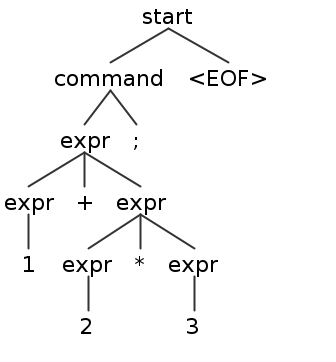
\includegraphics[width=.5\textwidth]{img1.png}
\end{center}

\end{document}
